% ARI v0.2 paper -- SKELETON. Bullets, figures, tables and equations; not prose.
% Every [TODO: ...] is an open decision or a sentence still to write.
% Numbers come from branch ilona/v02-reruns; each figure/table names its source file.
\documentclass{article}
\usepackage[preprint]{neurips_2026}
\usepackage[utf8]{inputenc}
\usepackage[T1]{fontenc}
\usepackage[hypertexnames=false]{hyperref}
\usepackage{url,booktabs,graphicx,amsmath,amssymb,xcolor,enumitem,multirow}
\usepackage{pgfplots}
\usepackage{tikz}
\usetikzlibrary{positioning,arrows.meta,shapes.misc}
\pgfplotsset{compat=1.18}
\setlist{nosep,leftmargin=*}

\definecolor{ari}{HTML}{0E6B73}
\definecolor{other}{HTML}{97A1AB}
\definecolor{benign}{HTML}{C47A22}
\definecolor{sig}{HTML}{B23A3A}
\newcommand{\todo}[1]{\textcolor{red}{\textbf{[TODO:} #1\textbf{]}}}
\newcommand{\src}[1]{\par\vspace{1pt}{\scriptsize\textcolor{gray}{source: \texttt{#1}}}}
\newcommand{\cond}[1]{\texttt{#1}}

\title{The AI Reproducibility Index: Detecting Meaningful Change in Model Outputs with Deterministic Codes \todo{title}}
\author{\todo{authors and affiliations}}

\begin{document}
\maketitle

\begin{abstract}
\begin{itemize}
  \item \textbf{Problem:} identical requests to the same model can return different outputs. Byte hashes flag every rounding difference, and task metrics (Recall@10, accuracy) average real changes away.
  \item \textbf{Method:} ARI turns each output vector (embedding or logits) into a deterministic code with the public SEMQ SDK, then compares codes across execution conditions. The headline score, ARI-R $=1-\bar\rho$, is the share of code positions unchanged, and it is comparable across model sizes.
  \item \textbf{Evidence that it is the right detector:} two pre-registered studies. At equal storage it catches every material change (48/48) and raises 0/336 false alarms, against 10--20 for float sketches and prefixes ($p\le 0.001$). Exploratory: SimHash raises 4/336 (not significant).
  \item \textbf{Findings:}
  \begin{itemize}
    \item bf16 changes the top-10 for up to 96\% of queries while Recall@10 moves significantly in 2 of 48 tests;
    \item ${\sim}1\%$ token change $\rightarrow$ 21--42\% of greedy generations differ, on two GPU types;
    \item a library upgrade silently loads 6/6 tested popular models in half precision, changing 15--100\% of codes;
    \item hosted embedding APIs range from bit-stable over six days to changing ${\sim}88\%$ of outputs on every call.
  \end{itemize}
  \item \todo{one-sentence implication; final abstract $\le$ 200 words}
\end{itemize}
\end{abstract}

% ===================================================================
\section{Introduction}\label{sec:intro}
\begin{itemize}
  \item \textbf{Motivation.} Retrieval, RAG and agents assume that the same input gives the same output. In practice, outputs change with process, hardware, batch shape, precision, library version and the serving backend. \todo{2--3 concrete incidents or citations}
  \item \textbf{Why existing checks fail:}
  \begin{itemize}
    \item \emph{Byte hashes} change on every harmless rounding difference (100\% of cross-device runs, \S\ref{sec:kernels}).
    \item \emph{Task metrics} average changes away (\S\ref{sec:blind}).
    \item \emph{Float distances} need a threshold, and at small storage they false-alarm (\S\ref{sec:select}).
  \end{itemize}
  \item \textbf{Idea.} Quantize each output into a fixed, versioned code. Small rounding noise does not cross a bin edge; a material change does. Codes are small, deterministic, and show \emph{which} coordinates moved.
  \item \textbf{Contributions:}
  \begin{enumerate}
    \item \textbf{ARI protocol and score:} conditions (Table~\ref{tab:conditions}), a fixed-range probe, and ARI-R, a dimension-normalized score (\S\ref{sec:method}).
    \item \textbf{Pre-registered validation:} two studies showing ARI separates material from benign change better than hashes and float sketches at equal storage (\S\ref{sec:select}).
    \item \textbf{Measurements:} self-hosted embedding and chat models, GPU kernels and settings, library defaults, and five hosted APIs (\S\ref{sec:blind}--\ref{sec:hosted}).
    \item \textbf{Open artifacts:} public SDK (\texttt{semq==1.0.0}), frozen inputs, signed reports, pre-registrations. \todo{repo URL, DOI}
  \end{enumerate}
\end{itemize}

% ===================================================================
\section{Method}\label{sec:method}

\begin{figure}[t]
\centering
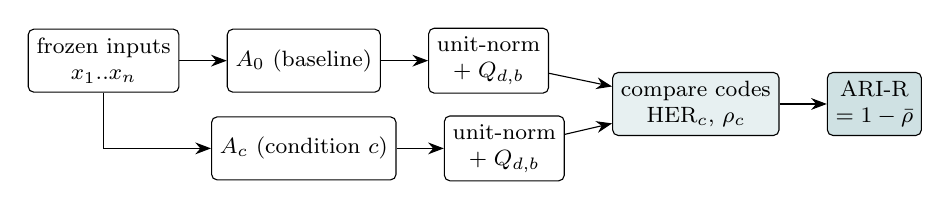
\begin{tikzpicture}[font=\footnotesize, box/.style={draw, rounded corners=2pt, align=center, minimum height=8mm, inner sep=3pt}, ->, >={Stealth[length=2mm]}]
  \node[box] (x) {frozen inputs\\$x_1..x_n$};
  \node[box, right=6mm of x] (a0) {$A_0$ (baseline)};
  \node[box, below=3mm of a0] (ac) {$A_c$ (condition $c$)};
  \node[box, right=6mm of a0] (q0) {unit-norm\\$+\;Q_{d,b}$};
  \node[box, right=6mm of ac] (qc) {unit-norm\\$+\;Q_{d,b}$};
  \node[box, right=8mm of q0, yshift=-5.5mm, fill=ari!10] (cmp) {compare codes\\HER$_c$, $\rho_c$};
  \node[box, right=6mm of cmp, fill=ari!20] (ari) {ARI-R\\$=1-\bar\rho$};
  \draw (x) -- (a0); \draw (x) |- (ac); \draw (a0) -- (q0); \draw (ac) -- (qc);
  \draw (q0) -- (cmp); \draw (qc) -- (cmp); \draw (cmp) -- (ari);
\end{tikzpicture}
\caption{ARI pipeline. A baseline run and a condition run encode the same frozen inputs. Each output row is normalized and quantized by the public SEMQ SDK; codes are compared position by position. \todo{add a small inset: one coordinate jittering inside a bin (no change) vs crossing an edge (change)}}
\label{fig:pipeline}
\end{figure}

\paragraph{System and conditions.}
\begin{itemize}
  \item System under test $A:\mathcal X\to\mathbb R^d$: an embedding model, or per-step logits under a fixed prefix (teacher-forced).
  \item Baseline run $A_0$ vs condition run $A_c$; each condition varies one execution axis (Table~\ref{tab:conditions}).
  \item Hosted APIs: the backend state is unobservable, so changes are \emph{associated} with a condition, not attributed to a cause.
\end{itemize}

\begin{table}[t]
\centering\footnotesize
\caption{Conditions. The core (\cond{proc}, \cond{conc}, \cond{time}) applies to any system, hosted or self-hosted; diagnostics need control of the stack. Labels follow the pre-registered rule (\S\ref{sec:select}): \emph{material} if numeric precision or quantization changes, \emph{benign} if only scheduling, shape or device changes.}
\label{tab:conditions}
\begin{tabular}{llll}
\toprule
condition & varies & where & label \\
\midrule
\cond{same} & immediate repeat, same process (control) & all & benign \\
\cond{proc} & fresh process or client & all & benign \\
\cond{conc} & 64-way concurrent burst vs calm pass & all & benign \\
\cond{time} & $\ge 24$\,h gap, same host & all & benign \\
\midrule
\cond{batch} & batch size 1/8/128/512 vs 32 & self-hosted & benign \\
\cond{threads} & 1 vs 4 CPU threads & self-hosted & benign \\
\cond{mach} & CPU $\leftrightarrow$ GPU, GPU $\leftrightarrow$ GPU (fp32) & self-hosted & benign \\
\cond{tf32} & TF32 matmul on vs off & self-hosted & material \\
\cond{prec} & bf16 / fp16 weights vs fp32 & self-hosted & material \\
\cond{lib} & library default load vs explicit fp32 & self-hosted & material (dtype changes) \\
\bottomrule
\end{tabular}
\end{table}

\paragraph{The probe (ARI-Canonical-v0.2).}
\begin{itemize}
  \item Normalize each row in binary64, cast to float32: $\hat a = a/\lVert a\rVert_2$.
  \item Fixed range set by the dimension alone (the SDK's \texttt{max\_magnitude}): $s_d = 2/\sqrt d$.
  \item Symbol per coordinate with $b$ magnitude bins (sign selects the half of the alphabet):
  \begin{equation}
    Q_{d,b}(\hat a)_j \;=\; b\cdot\mathbb 1[\hat a_j \ge 0] \;+\; \min\!\Big(\Big\lfloor \tfrac{b\,|\hat a_j|}{s_d}\Big\rfloor,\; b-1\Big),\qquad Q_{d,b}(\hat a)_j\in\{0,\dots,2b-1\}.
  \end{equation}
  \item Edges sit at multiples of $s_d/b$; magnitudes $|\hat a_j|\ge s_d$ saturate into the top bin. The bin index is computed in binary32 (round-to-nearest-even, no fused multiply-add), so every backend gives the same symbol (SDK \texttt{semq\_quant\_bin\_of\_magnitude}).
  \item ARI-R uses $b=2$ (2 bits per coordinate, $d/4$ bytes per vector). The logit probe uses $b=8$.
  \item Deterministic and bit-exact across platforms (SDK conformance vectors); the probe adds no disagreement of its own.
  \item \textbf{Why a fixed range:} the v0.1 probe calibrated $s$ on a data sample. Recalibrating on a different sample moved $s$ by 0.3--3.6\% and rewrote 60--100\% of codes for \emph{identical} vectors (\S\ref{sec:valid}).
\end{itemize}

\paragraph{Metrics.} For inputs $i=1..n$ and condition $c$, with codes $q_{0,i}=Q(\hat A_0(x_i))$, $q_{c,i}=Q(\hat A_c(x_i))$:
\begin{align}
  \mathrm{HER}_c &= \frac1n\sum_{i=1}^n \mathbb 1\!\left[q_{0,i}=q_{c,i}\right] && \text{(whole-code exact-match rate)}\\
  \rho_c &= \frac1{n\,d}\sum_{i=1}^n\sum_{j=1}^d \mathbb 1\!\left[q_{0,ij}\neq q_{c,ij}\right] && \text{(coordinate change rate)}\\
  \text{ARI-R} &= 1-\tfrac13\left(\rho_{\texttt{proc}}+\rho_{\texttt{conc}}+\rho_{\texttt{time}}\right) && \text{(headline; } \texttt{same} \text{ is a control)}
\end{align}
\begin{itemize}
  \item 95\% intervals: bootstrap over inputs, 1{,}000 resamples. \todo{state that they cover input sampling, not serving-environment realizations}
  \item \textbf{Report both.} $\rho$ (and ARI-R) is comparable across $d$; HER answers ``how many outputs changed at all''. Example: Voyage and OpenAI have equal ARI-R (0.99976) but HER 0.99 vs 0.93 (\S\ref{sec:hosted}).
\end{itemize}

\paragraph{ARI-D (decoding).}
\begin{itemize}
  \item \textbf{Self-hosted (logits).} ARI-D-Logit-v0.2: centre each logit row (remove the shift invariance of softmax), split it into fixed 65{,}536-wide chunks, normalize each chunk, and apply $Q_{\cdot,8}$. Teacher-forced on the baseline tokens, so every condition sees identical prefixes. Details in App.~\ref{app:logit}.
  \item \textbf{Hosted (text).} Rate of byte-identical completions over $k$ repeats per prompt, plus the mean relative position of the first divergence.
  \item \todo{decide whether ARI-D gets its own headline number or is reported per condition only}
\end{itemize}

% ===================================================================
\section{Is ARI a valid detector?}\label{sec:valid}

\paragraph{Dimension fairness.}
\begin{itemize}
  \item Inject the same relative noise ($\varepsilon=3\times10^{-3}$) into eight encoders' outputs, $d\in\{384,768,1024\}$.
  \item HER falls from 0.64 to 0.26--0.32 as $d$ grows; $\rho$ stays at 1.1--1.4$\times10^{-3}$ (Fig.~\ref{fig:dim}). So HER ranks models by size, not stability; ARI-R does not.
\end{itemize}

\begin{figure}[t]
\centering
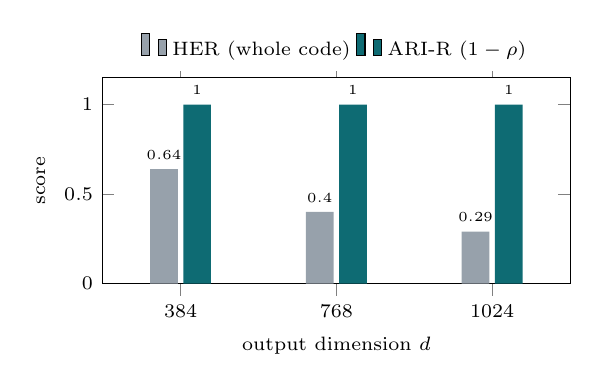
\begin{tikzpicture}
\begin{axis}[width=0.62\linewidth,height=4.2cm,ybar,bar width=10pt,ymin=0,ymax=1.15,
  symbolic x coords={384,768,1024},xtick=data,xlabel={output dimension $d$},ylabel={score},enlarge x limits=0.25,
  legend style={font=\scriptsize,at={(0.5,1.03)},anchor=south,legend columns=2,draw=none},
  nodes near coords,every node near coord/.append style={font=\tiny},
  ticklabel style={font=\scriptsize},label style={font=\scriptsize}]
\addplot[fill=other,draw=none] coordinates {(384,0.639) (768,0.40) (1024,0.29)};
\addplot[fill=ari,draw=none] coordinates {(384,0.9988) (768,0.9988) (1024,0.9987)};
\legend{HER (whole code),ARI-R ($1-\rho$)}
\end{axis}
\end{tikzpicture}
\caption{Same relative noise, different output sizes. Whole-code agreement penalizes larger $d$; the coordinate change rate does not. 1,024-d shows the midpoint of 0.26--0.32 across models.}
\label{fig:dim}
\src{scratchpad probe\_cmp (synthetic noise) \todo{commit the script and its output to experiments/}}
\end{figure}

\paragraph{Calibration dependence (why v0.2 fixes the range).}
\begin{itemize}
  \item v0.1 probe recalibrated on FiQA vs SciFact rows: $s$ moved 0.3--3.6\%, codes changed for 60--100\% of identical vectors (8 encoders).
  \item The fixed range has no calibration, so this failure mode is gone. \todo{one line on the version pin: spec ARI-Canonical-v0.2, \texttt{semq==1.0.0}}
\end{itemize}

% ===================================================================
\section{Selectivity: material vs benign change at matched storage}\label{sec:select}
\begin{itemize}
  \item \textbf{Question.} At equal stored bytes ($B=d/4$), which detector flags material changes and ignores benign ones?
  \item \textbf{Detectors} (App.~\ref{app:detectors}): ARI code; SHA-256 (32\,B); block hashes; fp16 prefix ($B/2$ coords); random-projection sketch ($B/4$ fp32 projections); full fp32 cosine ($4d$\,B, not matched). Exploratory: SimHash ($2d$ sign bits).
  \item \textbf{Study 1} (pre-registered, frozen 2026-10-07): 9 encoders, 600 episodes, 90 cells. The threshold is the largest score on the calibration half's benign cells; tested on the other half.
  \item \textbf{Study 2} (pre-registered, frozen 2026-10-12): 25 encoders (24 analyzed), 14 benign conditions, 336 benign + 48 material cells, CPU/A10G/T4/L4. \emph{Thresholds reused from Study~1}, so every cell is a test cell and 16 models are out-of-sample.
  \item \textbf{Primary test (Study 2):} paired one-sided exact sign test, code vs each matched detector on the same benign cells, Holm-adjusted.
\end{itemize}

\begin{table}[t]
\centering\footnotesize
\caption{Selectivity at matched storage. Study 1: test half (20 material, 30 benign cells), episode rates. Study 2: all cells. $p$: one-sided paired sign test vs the code on Study~2 benign cells (Holm for the two pre-registered comparisons).}
\label{tab:select}
\begin{tabular}{lrrrrrr}
\toprule
& & \multicolumn{2}{c}{Study 1} & \multicolumn{3}{c}{Study 2} \\
\cmidrule(lr){3-4}\cmidrule(lr){5-7}
detector & bytes & material & benign & material & benign & $p$ \\
\midrule
\textbf{ARI code} & $d/4$ & \textbf{1.000} & \textbf{0.000} & \textbf{48/48} & \textbf{0/336} & -- \\
SHA-256 & 32 & 0.000 & 0.000 & 0/48 & 0/336 & -- \\
block hashes & $d/4$ & 0.000 & 0.000 & 0/48 & 0/336 & -- \\
random sketch & $d/4$ & 1.000 & 0.035 & 48/48 & 10/336 & 0.001 \\
fp16 prefix & $d/4$ & 1.000 & 0.071 & 48/48 & 20/336 & $2\times10^{-6}$ \\
full cosine$^\dagger$ & $4d$ & 1.000 & 0.106 & 48/48 & 23/336 & $1\times10^{-7}$ \\
SimHash$^\ast$ & $d/4$ & 1.000 & 0.035 & 48/48 & 4/336 & 0.063 \\
\bottomrule
\end{tabular}\\[2pt]
{\scriptsize $^\dagger$not storage-matched, secondary. $^\ast$exploratory, added after both analyses, not pre-registered.}
\src{experiments/selectivity-confirmatory/results/results.json; experiments/selectivity-benign/results/\{results,exploratory\_simhash\}.json}
\end{table}

\begin{figure}[t]
\centering
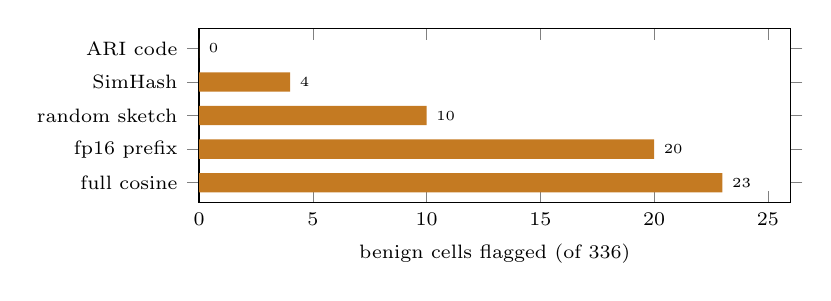
\begin{tikzpicture}
\begin{axis}[width=0.75\linewidth,height=3.8cm,xbar,bar width=7pt,xmin=0,xmax=26,
  symbolic y coords={full cosine,fp16 prefix,random sketch,SimHash,ARI code},ytick=data,
  xlabel={benign cells flagged (of 336)},nodes near coords,every node near coord/.append style={font=\tiny},
  ticklabel style={font=\scriptsize},label style={font=\scriptsize},enlarge y limits=0.15]
\addplot[fill=benign,draw=none] coordinates {(23,full cosine) (20,fp16 prefix) (10,random sketch) (4,SimHash) (0,ARI code)};
\end{axis}
\end{tikzpicture}
\caption{False alarms in Study 2. All detectors except the hashes caught 48/48 material cells. The other detectors' alarms concentrate on cross-device moves and four models (multilingual-e5-base, e5-large-v2, bge-m3, mpnet).}
\label{fig:select}
\end{figure}

\paragraph{Findings.}
\begin{itemize}
  \item Hashes cannot be selective: benign device changes alter every byte, so a zero-false-alarm threshold flags nothing (material 0/48).
  \item \textbf{Pre-registered claim supported:} at equal storage the code raises fewer benign alarms than the float sketch and the fp16 prefix, and catches every material cell. Code benign rate $\le$1.1\% (95\% Wilson upper bound).
  \item Quantized codes beat continuous ones. ARI vs SimHash is \emph{not} resolved: 4 discordant cells, all favouring ARI, $p=0.063$. ARI's case over SimHash is design: it localizes changes, needs no shared projection matrix, and follows a versioned spec.
  \item \textbf{Caveats:}
  \begin{itemize}
    \item One benign cell (MiniLM CPU vs A10G) scores exactly at the code threshold; it repeats the cell that set it.
    \item 81/336 benign cells moved $\ge$1 code symbol. Selectivity comes from the threshold, not from codes never changing.
    \item The code flags 53\% of material \emph{inputs}: it is a run-level detector.
  \end{itemize}
  \item \todo{one sentence: why sub-threshold invariance is the mechanism (bin edges vs jitter magnitude); maybe a histogram of per-input $\rho$ for benign vs material}
\end{itemize}

% ===================================================================
\section{Changes that task metrics miss}\label{sec:blind}

\paragraph{Retrieval.} 3 BEIR corpora (SciFact, NFCorpus, ArguAna) $\times$ 4 encoders (MiniLM, bge-large, e5-large, EmbeddingGemma~2); one setting changed at a time on an A10G; reference fp32 on CPU.

\begin{figure}[t]
\centering
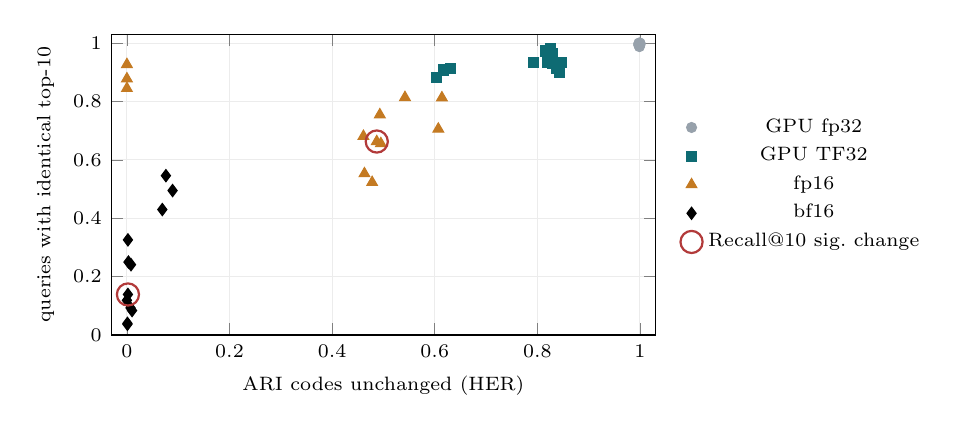
\begin{tikzpicture}
\begin{axis}[width=0.7\linewidth,height=5.4cm,xmin=-0.03,xmax=1.03,ymin=0,ymax=1.03,
  xlabel={ARI codes unchanged (HER)},ylabel={queries with identical top-10},
  legend style={font=\scriptsize,at={(1.03,0.5)},anchor=west,draw=none},
  ticklabel style={font=\scriptsize},label style={font=\scriptsize},grid=major,grid style={gray!15}]
\addplot[only marks,mark=*,mark size=1.8pt,color=other] coordinates {(1.000,0.994) (0.998,0.993) (0.999,0.993) (1.000,0.997) (0.999,0.988) (0.998,0.994) (0.998,0.997) (1.000,1.000) (0.998,1.000) (0.999,1.000) (0.999,0.997) (1.000,1.000)};
\addplot[only marks,mark=square*,mark size=1.8pt,color=ari] coordinates {(0.847,0.934) (0.793,0.934) (0.617,0.908) (0.844,0.898) (0.829,0.932) (0.838,0.913) (0.604,0.882) (0.830,0.963) (0.826,0.983) (0.630,0.913) (0.820,0.933) (0.816,0.973)};
\addplot[only marks,mark=triangle*,mark size=2.2pt,color=benign] coordinates {(0.000,0.878) (0.542,0.814) (0.461,0.681) (0.000,0.845) (0.607,0.706) (0.495,0.656) (0.478,0.523) (0.000,0.927) (0.614,0.813) (0.463,0.553) (0.493,0.755) (0.487,0.663)};
\addplot[only marks,mark=diamond*,mark size=2.2pt,color=black] coordinates {(0.076,0.546) (0.002,0.326) (0.000,0.119) (0.089,0.495) (0.002,0.139) (0.010,0.084) (0.001,0.040) (0.069,0.430) (0.003,0.250) (0.001,0.037) (0.008,0.241) (0.007,0.093)};
\addplot[only marks,mark=o,mark size=4pt,color=sig,thick] coordinates {(0.487,0.663) (0.002,0.139)};
\legend{GPU fp32,GPU TF32,fp16,bf16,Recall@10 sig.\ change}
\end{axis}
\end{tikzpicture}
\caption{48 retrieval runs (12 per setting). Codes and per-query rankings move together; Recall@10 changes significantly in only 2 runs (circled: bf16, NFCorpus/bge-large, $-0.2$ pts; fp16, SciFact/EmbeddingGemma~2, $-1.5$ pts). Under bf16, as few as 4\% of queries keep their top-10.}
\label{fig:retrieval}
\src{s3 ari-v02-reruns/casestudies\{,\_rest\}/regime\_matrix\_*\_b2.json \todo{commit these JSONs to the repo}}
\end{figure}

\begin{itemize}
  \item Recall@10 is an average over relevance judgments; a reordered top-10 keeps the average when the relevant documents stay in. \todo{1 sentence why; cite}
  \item MiniLM changes \emph{every} code under fp16 on all three corpora (HER 0.000), while larger models keep ${\sim}$0.5. \todo{explain before submission: fp16 range in a small model? check activations}
\end{itemize}

\paragraph{Decoding.} Three 7--8B instruct models, 48 prompts, 48 greedy tokens; L40S and H100.

\begin{figure}[t]
\centering
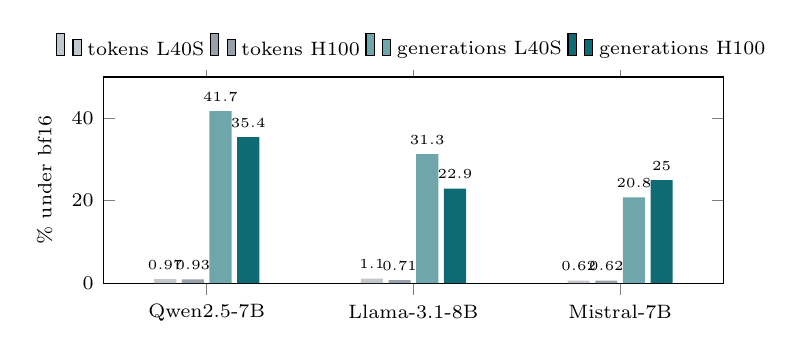
\begin{tikzpicture}
\begin{axis}[width=0.78\linewidth,height=4.2cm,ybar,bar width=8pt,ymin=0,ymax=50,
  symbolic x coords={Qwen2.5-7B,Llama-3.1-8B,Mistral-7B},xtick=data,ylabel={\% under bf16},
  legend style={font=\scriptsize,at={(0.5,1.03)},anchor=south,legend columns=4,draw=none},
  nodes near coords,every node near coord/.append style={font=\tiny},
  ticklabel style={font=\scriptsize},label style={font=\scriptsize},enlarge x limits=0.25]
\addplot[fill=other!60,draw=none] coordinates {(Qwen2.5-7B,0.97) (Llama-3.1-8B,1.10) (Mistral-7B,0.62)};
\addplot[fill=other,draw=none] coordinates {(Qwen2.5-7B,0.93) (Llama-3.1-8B,0.71) (Mistral-7B,0.62)};
\addplot[fill=ari!60,draw=none] coordinates {(Qwen2.5-7B,41.7) (Llama-3.1-8B,31.3) (Mistral-7B,20.8)};
\addplot[fill=ari,draw=none] coordinates {(Qwen2.5-7B,35.4) (Llama-3.1-8B,22.9) (Mistral-7B,25.0)};
\legend{tokens L40S,tokens H100,generations L40S,generations H100}
\end{axis}
\end{tikzpicture}
\caption{Under bf16, ${\le}1.1\%$ of teacher-forced tokens change, but 21--42\% of complete greedy generations differ, on both GPUs.}
\label{fig:decoding}
\src{s3 ari-v02-reruns/\{l40s,l40s\_retry,h100\_extra\}/decoding\_matrix\_*\_gpu.json}
\end{figure}

\begin{table}[t]
\centering\footnotesize
\caption{ARI-D logit codes see changes before the text does. Ranges over 3 models $\times$ 2 GPUs (L40S, H100), vs fp32.}
\label{tab:decoding}
\begin{tabular}{lrr}
\toprule
condition & logit codes unchanged & generations identical \\
\midrule
fresh process, 1 thread & 1.000 & 48/48 \\
padded batch of 4 & 0.25--0.78 & 48/48 \\
TF32 on & 0.000 & 48/48 \\
fp16 weights & 0.000 & 43--46/48 \\
bf16 weights & 0.000 & 28--38/48 \\
\bottomrule
\end{tabular}
\end{table}

\begin{itemize}
  \item Compounding: one flipped token early changes the rest of the generation. \todo{plot first-divergence position vs top-2 margin; data in decoding JSONs (median margin at flipped tokens 0.04--0.06 vs 3.2--4.2 overall)}
\end{itemize}

% ===================================================================
\section{Where changes come from}\label{sec:kernels}

\paragraph{Same kernel, same output.} Every self-hosted repeat that keeps the kernel fixed is bit-identical: CPU (9 encoders, including at a 24--30\,h gap), and A10G and H100 in a fresh process with TF32 on or off and determinism on or off (8/8 encoders each).

\paragraph{Different kernel: bytes change, codes almost never.}
\begin{table}[t]
\centering\footnotesize
\caption{Benign kernel changes in Study 2 (24 encoders, 1,000 inputs per cell, fp32). Raw bytes change for nearly every input under GPU batch or device changes; codes move by at most ${\sim}2$ positions in 384{,}000.}
\label{tab:kernels}
\setlength{\tabcolsep}{4pt}
\begin{tabular}{lrrrr}
\toprule
change & \shortstack[r]{inputs w/\\byte change} & \shortstack[r]{cells w/\\byte change} & \shortstack[r]{cells w/\\code change} & max $\rho$ \\
\midrule
fresh process (CPU, GPU) & 0.000 & 0/24 & 0/24 & 0 \\
1 vs 4 CPU threads & 0.005 & 15/24 & 0/24 & 0 \\
CPU batch 8 / 128 & 0.14 / 0.08 & 22 / 24 & 0 / 2 & $2.6\times10^{-6}$ \\
GPU batch 1 / 8 / 128 / 512 & 0.96--1.00 & 24/24 & 7--12 & $5.2\times10^{-6}$ \\
CPU $\leftrightarrow$ A10G / T4 / L4 & 1.000 & 24/24 & 8--11 & $5.2\times10^{-6}$ \\
A10G $\leftrightarrow$ T4 / L4 & 0.92--1.00 & 24/24 & 4--11 & $5.2\times10^{-6}$ \\
\bottomrule
\end{tabular}
\src{experiments/selectivity-benign/results/results.json (per-cell scores)}
\end{table}

\paragraph{Settings that change outputs.}
\begin{itemize}
  \item \textbf{Precision} dominates: a fresh bf16 load keeps 0.1--7.3\% of codes on CPU (9 encoders); fp16/bf16 on GPU in Fig.~\ref{fig:retrieval}.
  \item \textbf{TF32} changes 15--40\% of codes vs off (A10G), with no change in Recall@10 or any generation. It is a configuration difference, not nondeterminism. PyTorch's default is off for matmul.
  \item \textbf{TF32 $\times$ batch} (H100): batch changes move codes for some encoders only when TF32 is on (Table~\ref{tab:h100}).
  \item \textbf{Library defaults} (Fig.~\ref{fig:lib}): 35 of the top-200 HF embedding models declare half precision. transformers~5 loads it by default (v4 loaded fp32), changing 15--100\% of codes. One model (gte-multilingual-base) no longer runs.
  \item \textbf{Broken outputs:} EmbeddingGemma~2 in fp16 emits NaN vectors for 25/5{,}183 SciFact docs (0.48\%; identical in two runs), 9/3{,}633 NFCorpus and 1/8{,}674 ArguAna. The SciFact case gives the largest Recall@10 drop observed ($-1.5$ pts).
\end{itemize}

\begin{table}[t]
\centering\footnotesize
\caption{H100 batch invariance: codes unchanged vs batch 32 under the same settings, 9 encoders, 1,000 inputs. Most encoders stay ${\ge}0.996$ with TF32 on; mpnet, nomic and EmbeddingGemma~2 set the minima.}
\label{tab:h100}
\setlength{\tabcolsep}{4pt}
\begin{tabular}{lrrrrr}
\toprule
& same batch, new process & b=1 & b=8 & b=128 & b=512 \\
\midrule
TF32 off (det.\ on/off) & 1.000 & 0.999--1.000 & 0.999--1.000 & 0.999--1.000 & 0.999--1.000 \\
TF32 on & 1.000 & 0.792--1.000 & 0.830--1.000 & 0.864--1.000 & 0.825--1.000 \\
\bottomrule
\end{tabular}
\src{s3 ari-v02-reruns/h100/batch\{,\_gemma\}/summary.json}
\end{table}

\begin{figure}[t]
\centering
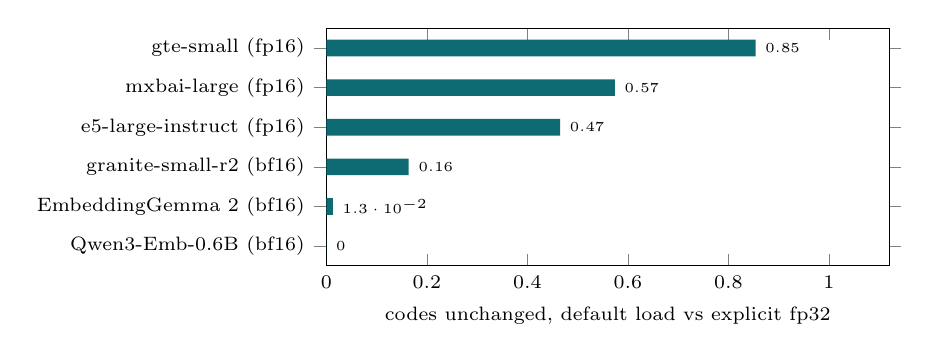
\begin{tikzpicture}
\begin{axis}[width=0.72\linewidth,height=4.6cm,xbar,bar width=6pt,xmin=0,xmax=1.12,
  symbolic y coords={qwen,gemma,granite,e5i,mxbai,gte},ytick=data,
  yticklabels={Qwen3-Emb-0.6B (bf16),EmbeddingGemma 2 (bf16),granite-small-r2 (bf16),e5-large-instruct (fp16),mxbai-large (fp16),gte-small (fp16)},
  xlabel={codes unchanged, default load vs explicit fp32},nodes near coords,every node near coord/.append style={font=\tiny},
  ticklabel style={font=\scriptsize},label style={font=\scriptsize},enlarge y limits=0.1]
\addplot[fill=ari,draw=none] coordinates {(0.000,qwen) (0.013,gemma) (0.164,granite) (0.465,e5i) (0.574,mxbai) (0.854,gte)};
\end{axis}
\end{tikzpicture}
\caption{The \cond{lib} condition on an H100 with transformers 5.19: the same user code, \texttt{SentenceTransformer(model\_id)}, now loads the checkpoint's declared half precision. gte-multilingual-base fails to run (not shown). EmbeddingGemma~2 requires transformers~5, so for it this is the default rather than a change.}
\label{fig:lib}
\src{s3 ari-v02-reruns/h100\_extra/lib\_fix/*.json; HF scan hf\_dtype\_scan.json \todo{commit both}}
\end{figure}

% ===================================================================
\section{Hosted systems}\label{sec:hosted}

\begin{table}[t]
\centering\footnotesize
\caption{Hosted embedding APIs, 1,000 frozen inputs. HER per condition; \cond{time} 148--150\,h after the baseline; \cond{conc}: 64-way burst. \cond{batch} (diagnostic): same texts sent batched vs one per request.}
\label{tab:api}
\begin{tabular}{lrrrrrr}
\toprule
API & \cond{same} & \cond{proc} & \cond{conc} & \cond{time} & \cond{batch} & ARI-R \\
\midrule
gemini-embedding-001 & 1.000 & 1.000 & 1.000 & 1.000 & -- & 1.000000 \\
voyage-4-large & 0.997 & 0.990 & 0.994 & 0.996 & 0.996 & 0.999758 \\
text-embedding-3-large & 0.934 & 0.957 & 0.943 & 0.925 & 0.063 & 0.999760 \\
embed-v4.0 & 0.116 & 0.124 & 0.165 & 0.123 & 0.058 & 0.989757 \\
mistral-embed & \multicolumn{6}{c}{\todo{rerun; times out under the 16-way burst}} \\
\bottomrule
\end{tabular}
\src{scratch api\_panel/submissions/*.json \todo{commit signed reports}}
\end{table}

\begin{itemize}
  \item Stability is per product, not per provider: Gemini's embedding API is bit-stable over six days; Gemini chat (below) is not.
  \item Cohere: ${\sim}$88\% of outputs change on every call, but no more after six days: constant noise, not drift.
  \item OpenAI: stable per request, but batching changes 94\% of codes. \todo{practitioner note: batch shape is part of the contract}
  \item \textbf{Hosted chat (ARI-D, text):} gemini-3.6-flash, temperature 0, fixed seed, 100 prompts $\times$ 8. Identical pairs: 0.626 within day 1, 0.564 within day 2, 0.594 [0.559, 0.633] across 29.8\,h. No time effect beyond within-batch variation.
  \item \todo{OpenRouter gateway control and Mistral chat (blocked: key, quota); decide whether the gateway case stays}
  \item \textbf{Deviation from v0.1:} Voyage \cond{conc} 0.209 $\rightarrow$ 0.994. The probe changed too, so we cannot attribute the difference. \todo{keep in appendix only?}
\end{itemize}

% ===================================================================
\section{Discussion}\label{sec:discussion}
\paragraph{Recommendations for practitioners.}
\begin{itemize}
  \item Pin precision explicitly (\texttt{torch\_dtype}) and assert it after loading; do not rely on library defaults.
  \item Treat TF32, batch shape and hardware as part of the deployment contract; record them with the index.
  \item Store ARI codes ($d/4$ bytes) alongside embeddings; compare after every upgrade. A hash will always differ across hardware; a task metric will usually say ``no change''.
  \item For hosted APIs, measure \cond{same} first: some services are noisy on every call.
\end{itemize}
\paragraph{What ARI is not.}
\begin{itemize}
  \item Not a quality metric: a code change says outputs moved, not that they got worse.
  \item Not a per-output detector: it reliably flags runs, and about half the changed inputs within a run.
  \item Not causal on hosted systems.
\end{itemize}
\paragraph{Limitations.}
\begin{itemize}
  \item One input set (1,000 frozen texts, English-heavy). \todo{language mix}
  \item The threshold was set on 9 encoders and carried to 16 more; zero margin on one benign cell.
  \item Hosted results are a snapshot; services change without notice.
  \item ARI vs SimHash unresolved; a larger pre-registered study is future work.
  \item \textbf{Correction:} v0.1 reported that TF32-on runs disagree across processes. That came from a harness bug (the worker process did not apply TF32). Corrected runs repeat exactly (App.~\ref{app:errata}).
\end{itemize}

\section{Related work}\label{sec:related}
\begin{itemize}
  \item Nondeterminism in deep learning and batch invariance. \todo{cite: PyTorch reproducibility docs; batch-invariant kernels work; floating-point non-associativity}
  \item LLM serving nondeterminism and temperature-0 variance. \todo{cite}
  \item Hashing and sketching: SHA-256, LSH/SimHash (Charikar 2002), random projections. \todo{cite}
  \item Embedding quantization and compact codes: binary embeddings, PQ, quantized hyperdimensional representations (qFHRR). \todo{cite; one sentence each}
  \item ML reproducibility checklists and benchmarks. \todo{cite}
\end{itemize}

\section{Conclusion}
\begin{itemize}
  \item \todo{3 sentences: deterministic codes detect what hashes over-flag and metrics miss; validated by pre-registration; changes come from configuration, not randomness, and from silent defaults}
\end{itemize}

\paragraph{Reproducibility statement.} \todo{SDK version and pin; frozen input hash; pre-registration commits (565aa57, 72f1247); signed reports (KMS key id); hardware list; S3 $\rightarrow$ repo migration of raw results}

% ===================================================================
\appendix
\section{Changes from v0.1}\label{app:changes}
\begin{table}[h]
\centering\scriptsize
\begin{tabular}{p{2.3cm}p{4.1cm}p{5.2cm}}
\toprule
area & v0.1 & v0.2 \\
\midrule
SDK & private pre-release build & public \texttt{semq==1.0.0}, pinned \\
probe range & calibrated on a sample (99th pct.) & fixed $2/\sqrt d$ \\
headline score & ARI-HER (+ noise-scale $\hat\sigma$) & ARI-R $=1-\bar\rho$; HER reported alongside \\
logit probe & embedding probe on raw logits & centred, 65,536-wide chunks, 8 bins \\
precision & library default & set and asserted per capture \\
\cond{time} (self-hosted) & not a true 24\,h gap & enforced $\ge$24\,h, same host \\
models & 8 encoders & + EmbeddingGemma 2; 25 in Study 2 \\
evidence & exploratory & two pre-registered studies \\
retrieval & SciFact, 1 encoder, 8 bins & 3 corpora $\times$ 4 encoders, 2 bins \\
TF32 claim & ``breaks cross-process repeatability'' & bug; corrected (App.~\ref{app:errata}) \\
removed & ARI-E, 15-hop walk, regions modules & out of scope or unsourced \\
\bottomrule
\end{tabular}
\end{table}

\section{Logit probe details}\label{app:logit}
\begin{itemize}
  \item Centre: $\ell \leftarrow \ell - \tfrac1V\sum_v \ell_v$. Chunk width $W=65{,}536$ (SDK maximum dimension); normalize each chunk; $Q_{W,8}$.
  \item Exploratory comparison on Qwen2.5-0.5B: catches 82.5\% of GPU-fp32 changes (vs 71.3\% for the v0.1 probe). A constant shift of $+3$ changes 1.7\% of codes (vs 100\%). Spearman 0.84--0.86 with centred drift. \todo{commit logit\_cmp outputs}
\end{itemize}

\section{Detector definitions}\label{app:detectors}
\begin{itemize}
  \item fp16 prefix: first $B/2$ coordinates in fp16; statistic $\tfrac{1}{k}\sum_j |a_j-a'_j|$.
  \item Sketch: $P\in\mathbb R^{d\times B/4}$, $P_{jk}\sim\mathcal N(0,1/k)$, seed $d$; statistic $\lVert (a-a')P\rVert_2$.
  \item SimHash: $R\in\mathbb R^{d\times 2d}$ Gaussian, seed $10^4+d$; statistic: fraction of $\mathrm{sign}(aR)$ bits flipped.
  \item Block hashes: $B/32$ SHA-256 digests over contiguous coordinate blocks; statistic: fraction of blocks changed.
\end{itemize}

\section{Pre-registrations and deviations}\label{app:prereg}
\begin{itemize}
  \item Study 1: frozen \texttt{565aa57}. Deviation: CPU host out of memory at 2 parallel captures; resumed at 1; 2 captures repeated. Note added after results: the code's benign interval [0,0] understates uncertainty (Wilson upper bound 0.114).
  \item Study 2: frozen \texttt{72f1247}. Amendment before capture: GPU regions. Qwen3-Embedding-0.6B dropped (batch 512 out of memory on A10G), as pre-registered.
\end{itemize}

\section{Errata: TF32 cross-process measurement}\label{app:errata}
\begin{itemize}
  \item Bug: the \cond{proc} worker in \texttt{gpu\_capture.py} did not apply TF32 or determinism flags, so ``TF32 on, new process'' compared on vs off. Present since the first harness commit; fixed in \texttt{a617e48}.
  \item Corrected: A10G and H100, 8 encoders, TF32 on/off $\times$ determinism on/off: \cond{proc} HER 1.000 in all 32 cells per GPU.
  \item Superseded claims: v0.1 ``TF32 alone breaks GPU reproducibility'' and ``the deterministic flag had no effect''. \todo{list exact v0.1 sentences}
\end{itemize}

\section{Hardware and software}\label{app:stack}
\begin{itemize}
  \item CPU: AWS c7i.2xlarge. GPUs: A10G (g5), T4 (g4dn), L4 (g6), L40S (g6e), H100 80GB (p5.4xlarge capacity block).
  \item Python 3.12; torch 2.6.0 (cu124), transformers 4.57.6, sentence-transformers 4.1.0. EmbeddingGemma 2: torch 2.14.1, transformers 5.19.0, sentence-transformers 6.1.0.
  \item \todo{note: on Hopper with the DLAMI, system CUDA 13.2 libraries on LD\_LIBRARY\_PATH break torch 2.14.1's cuDNN; we unset it}
\end{itemize}

\end{document}
